%!TEX root = ../PTC-LibUG.tex

\chapter{Geometric Routines}
\label{cha:geometry}

\fxnote{Need to proof-read geometric formulas.}
\fxnote{Could we make the red italic type less glaring?}

\index{routines!geometric}
\index{geometric routines!described}
%
\PTC's geometric routines are divided into three categories:
\begin{itemize}
  \item affine routines on pure geometry,
  \item affine routines on computer objects,
  \item dynamical routines.
\end{itemize}

Mandatory arguments for the geometric routines are in \ptc{regular
black} type.  Optional arguments are in \ptc{\textit{\textcolor{red}{red
italic}}} type.


\section{Affine Routines on Pure Geometry}

\index{affine routines!on pure geometry}
\index{routines!affine}
\index{affine basis!geometric routines}
\index{global frame!geometric routines}
%
Affine routines on pure geometry act on a pure geometrical affine basis:
\ptc{A(3)} and \ptc{V(3,3)} where \ptc{A} represents the coordinates of a
point in the global frame, and \ptc{V(3,3)} the coordinates of a triad of vectors.


\subsection{Theory}
\label{sub:Theory-Affine-Routines}

\index{affine routines!theory}
%
Consider a point $a$ and vector basis $(v_1,v_2,v_3)$ attached
to a solid (a magnet, for example). See \fref{Rotating-point-a}.

\begin{figure}[ht]
  \centering
  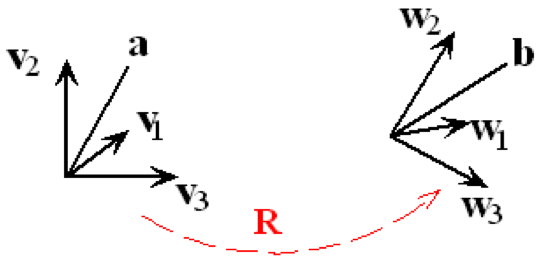
\includegraphics{illustrations/geo-routines-1}
  \caption{Rotating point $a$ and vector basis $(v_1,v_2,v_3)$ by $R$.}
  \label{fig:Rotating-point-a}
\end{figure}

The vector $a$ can be expressed as follows:
\begin{equation*}
  a = \sum_i  a_i v_i.
\end{equation*}

The basis vectors $v_i$ can be expressed in terms of a global basis, that is, \PTC's global frame:
\begin{equation*}
  v_i = \sum_j V_{ij} e_j.
\end{equation*}
 
Suppose we rotate the solid by a rotation $R$ defined by its action on the basis
$(v_1,v_2,v_3)$:
\begin{equation*}
  w_i = R v_i = \sum_j R_{ij} v_j.
\end{equation*}

Then we ask the following question: what are the components of $w_i$ in the global basis $(e_1,e_2,e_3)$ in terms of the component array $V_{ij}$?

Note: The components of $b$ in the frame $(w_1,w_2,w_3)$,
which is the image of $a$ upon rotation of the magnet, are
also given $a_i$ because this point is fixed in the magnet.

Solution:
\begin{equation*}
 w_i = R v_i = \sum_j R_{ij} v_j = \sum_{jk} R_{ij} V_{jk} e_k = \sum_k W_{ik} e_k.
\end{equation*}

Thus we have
\begin{equation*}
  W = RV.
\end{equation*}

The components of the vector $b$ in the global frame are then
\begin{equation*}
  b_k = \sum_{ij} a_i R_{ij} V_{jk} e_k
  \rightarrow b = (RV)^t a.
\end{equation*}

We now address a slightly harder problem, which is essential in \PTC.
The rotation $R$, instead of being defined in the frame $(v_1,v_2,v_3)$,
might be defined on a totally different frame $(u_1,u_2,u_3)$:
\begin{equation*}
  u_i = \sum_k U_{ik} e_k.
\end{equation*}
Therefore, prior to rotating the basis $(v_1,v_2,v_3)$, we must
express it in the frame $(u_1,u_2,u_3)$:
\begin{equation*}
  a = \sum_{ik} a_i V_{ik} e_k
    = \sum_{ikn} a_i V_{ik} U^{-1}_{kn} u_n
    = \sum_{ikn} a_i V_{ik} U_{nk} u_n.
\end{equation*}

We can now apply the rotation $R$ defined on the basis $(u_1,u_2,u_3)$:
\begin{equation*}
  b = \sum_{iknm} a_i V_{ik} U_{nk} R_{nm} u_m
    = \sum_{iknm} a_i V_{ik} U_{nk} R_{nm} U_{mk} e_k.
\end{equation*}

Thus the final result of $W$ is:
\begin{equation*}
  W = VU^t RU
\end{equation*}

The point $b$ in global coordinates is:
\begin{equation*}
  b_i = \sum_k a_i W_{ik}
  \rightarrow b = (VU^t RU)^t a.
\end{equation*}

Notice that if $V=U$, we regain the previous result.

\PTC\ factors the rotation $R$ in the form
\begin{equation*}
  R = R_z R_y R_x
\end{equation*}

Using local variables results in the need to go back and forth between frames.
The magnets must be placed within the global frame. However, the tracking is
in local variables. We need routines that are able to connect geometrically
both points of view.


\subsection{Descriptions of the Routines}

This section describes the affine routines on pure geometry.


\subsubsection{GEO\_ROT}

\begin{ptccode}
GEO_ROT(V(3, 3),W(3, 3),A(3),B(3),ANG(3)\textit{\textcolor{red}{,BASIS(3,3)}})
\end{ptccode}

\index{routine!\ptc{GEO\_ROT}}
\index{GEO\_ROT@\ptc{GEO\_ROT}!routine}
%
This routine exactly reproduces the theory in the previous section.

\ptc{BASIS} is an optional variable, which is set equal to the $U$ described
in Section~\ref{sub:Theory-Affine-Routines}.

The real array \ptc{ANG(3)} is used to define $R$:
\begin{equation*}
R = R_z (ang(3)) R_y (ang(2)) R_x (ang(1))
\end{equation*}

\begin{ptccode}
GEO_ROT(V(3, 3),W(3, 3),ANG(3)\textit{\textcolor{red}{,BASIS(3,3)}})
\end{ptccode}

This routine is the same as the previous routine except that
\ptc{A} and \ptc{B} are not needed.

\begin{ptccode}
GEO_ROT(V(3, 3),A(3),ANG(3),I\textit{\textcolor{red}{,BASIS(3,3)}})
\end{ptccode}

Here the final $W$ and $B$ are copied back into $V$ and $A$. The
integer \ptc{I} can be $\pm1$ to produce the inverse rotation: $R^{\pm1}$.

\begin{ptccode}
GEO_ROT(V(3, 3),ANG(3),I\textit{\textcolor{red}{,BASIS(3,3)}})
\end{ptccode}

This routine is the same as the previous routine without the \ptc{A} vector.


\subsubsection{GEO\_TRA}

\begin{ptccode}
GEO_TRA(A(3),V(3, 3) (3),D,I)
\end{ptccode}

\index{routine!\ptc{GEO\_TRA}}
\index{GEO\_TRA@\ptc{GEO\_TRA}!routine}
%
\ptc{A} is translated by $\pm$ \ptc{D} expressed in the basis \ptc{V}; \ptc{I} = $\pm1$.
\begin{equation*}
  \text{result} = \sum_{ij} (a_j e_j \pm d_i V_{ij} e_j)
\end{equation*}

The result is put back in \ptc{A}, that is:
\begin{equation*}
  A \leftarrow A \pm V^t D
\end{equation*}


\subsubsection{Rotating and Translating the Frames of a Magnet}

\begin{ptccode}
ROTATE_FRAME(F,OMEGA,ANG,ORDER\textit{\textcolor{red}{,BASIS(3,3)}})
\end{ptccode}

\index{translation routines!described}
\index{rotation routines!described}
\index{routine!\ptc{ROTATE\_FRAME}}
\index{ROTATE\_FRAME@\ptc{ROTATE\_FRAME}!routine}
%
\ptc{F} is of type \ptc{magnet\_frame} and contains three affine frames tied
to the magnet.
\begin{equation*}
F = \lbrace ( F \% A(3), F \% ENT(3) ), ( F \% O(3), F \% MID(3) ), ( F \% B(3), F \% EXI(3) ) \rbrace
\end{equation*}

The entire content of \ptc{F} is rotated as shown in \fref{Rotating-and-translating}.

\begin{figure}[ht]\forceversofloat
  \centering
  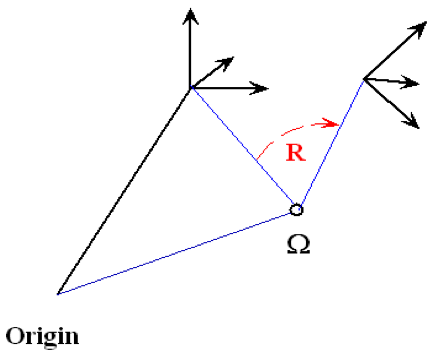
\includegraphics{illustrations/geo-routines-2}
  \caption{Rotating and translating the frames of a magnet.}
  \label{fig:Rotating-and-translating}
\end{figure}

\index{routine!\ptc{TRANSLATE\_FRAME}}
\index{TRANSLATE\_FRAME@\ptc{TRANSLATE\_FRAME}!routine}
%
\begin{ptccode}
TRANSLATE_FRAME(F,D,ORDER\textit{\textcolor{red}{,BASIS(3,3)}})

CALL CHANGE_BASIS(D,BASIS,DD,GLOBAL_FRAME)

P%A = P%A + ORDER * DD
P%B = P%B + ORDER * DD
P%O = P%O + ORDER * DD
\end{ptccode}

The frame is simply translated by \ptc{D}. The translation \ptc{D} is expressed
in \ptc{BASIS} if present.


\subsubsection{CHANGE\_BASIS}

\index{routine!\ptc{CHANGE\_BASIS}}
\index{CHANGE\_BASIS@\ptc{CHANGE\_BASIS}!routine}
%
\begin{ptccode}
CHANGE_BASIS(A(3),V(3,3),B(3),W(3,3))
\end{ptccode}

The component vector \ptc{A}, expressed in the basis \ptc{V}, is re-expressed
as \ptc{B} using basis \ptc{W}. \ptc{B} is the output of this subroutine.
\begin{equation*}
  \sum_{ik} a_i V_{ik} e_k = \sum_{ik} b_i W_{ik} e_k
  \rightarrow b = WV^t a.
\end{equation*}


\subsubsection{COMPUTE\_ENTRANCE\_ANGLE}

\index{routine!\ptc{COMPUTE\_ENTRANCE\_ANGLE}}
\index{COMPUTE\_ENTRANCE\_ANGLE@\ptc{COMPUTE\_ENTRANCE\_ANGLE}!routine}
%
\begin{ptccode}
COMPUTE_ENTRANCE_ANGLE(V(3,3),W(3,3),ANG(3))
\end{ptccode}

\index{rotation!order of}
%
This is a crucial routine. Given two frames \ptc{V} and \ptc {W}, which most likely
represent a magnet or a beam line, the routine computes a rotation
$R$ in the standard \PTC\ order, that is,
\begin{equation*}
  R = R_z (\ptc{ang(3)}) R_y (\ptc{ang(2)}) R_x (\ptc{ang(1)})
\end{equation*}
such that \ptc{V} is transformed into \ptc{W}. It is the reverse routine from \ptc{GEO\_ROT}.


\subsubsection{FIND\_PATCH\_B}

\index{routine!FIND\_PATCH\_B@\ptc{FIND\_PATCH\_B}}
\index{FIND\_PATCH\_B@\ptc{FIND\_PATCH\_B}!routine}
\index{patching!FIND\_PATCH\_B@\ptc{FIND\_PATCH\_B} routine}
\index{patch!inserting}
%
This routine connects the affine frame \ptc{A,V} to the affine frame \ptc{B,W}.

\begin{ptccode}
FIND_PATCH_B(A(3),V(3,3),B(3),W(3,3),D(3),ANG(3))
\end{ptccode}

\begin{ptccode}
SUBROUTINE FIND_PATCH_B(A,V,B,W,D,ANG)
  !\ FINDS PATCH BETWEEN V AND W : INTERFACED LATER FOR FIBRES
  IMPLICIT NONE
  REAL(DP), INTENT(INOUT) ::\ V(3,3),W(3,3)
  REAL(DP), INTENT(INOUT) ::\ A(3),B(3),D(3),ANG(3)
  CALL COMPUTE_ENTRANCE_ANGLE(V,W,ANG)
  D=B-A; CALL CHANGE_BASIS(D,GLOBAL_FRAME,D,W);
END SUBROUTINE FIND_PATCH_B
\end{ptccode}

The above code is a simple example of the usage of the geometric routines.
This geometric routine is very close to the dynamical set up of \PTC. Patches
are written as an ``x'' rotation, a ``y'' rotation, a ``z'' rotation, followed by a
translation (transverse + drift). Note that the translation $D = B - A$ between
is expressed in the final frame $W$. This is normal if dynamical rotations
precede the translations.


\subsubsection{FIND\_INVERSE\_PATCH}

\index{routine!\ptc{INVERSE\_FIND\_PATCH}}
\index{INVERSE\_FIND\_PATCH@\ptc{INVERSE\_FIND\_PATCH}!routine}
\index{patching!\ptc{INVERSE\_FIND\_PATCH} routine}
\index{patch!inserting}
%
This routine is the precise inverse of the \ptc{FIND\_PATCH\_B} routine.
The affine frame \ptc{B,W} is the output.

\begin{ptccode}
INVERSE_FIND_PATCH(A(3),V(3,3),D(3),ANG(3),B(3),W(3,3))
\end{ptccode}

\begin{ptccode}
SUBROUTINE INVERSE_FIND_PATCH(A,V,D,ANG,B,W)
  !\ USED IN MISALIGNMENTS OF SIAMESE
  IMPLICIT NONE
  REAL(DP), INTENT(INOUT)::\ V(3,3),W(3,3)
  REAL(DP), INTENT(INOUT)::\ A(3),B(3),D(3),ANG(3)
  REAL(DP) ::\  DD(3)
  W=V
  CALL GEO_ROT(W,ANG,1,BASIS=V)
  CALL CHANGE_BASIS(D,W,DD,GLOBAL_FRAME)
  B=A+DD
END SUBROUTINE INVERSE_FIND_PATCH
\end{ptccode}


\section{Affine Routines on Computer Objects}

\index{affine routines!on computer objects}
\index{routines!affine}
\index{affine basis!geometric routines}
%
Affine routines on \PTC's computer objects act on the affine bases of magnets,
siamese, girders, integration nodes, and fibres. These objects contain
a myriad of affine bases to help us locate the trajectories in 3-D.

Within this category are two subcategories:
\begin{itemize}
  \item \emph{Affine Routines on Fibrous Structures:} Displacements
that correspond to the design positioning and thus requiring patching.
  \item \emph{Misalignment Routines:} Misalignments representing errors
that do not require patching. The misalignments displace the magnet away
from a fibre that contains it. The misalignments also displace girders
away from their original position.
\end{itemize}


\subsection{Affine Routines on Fibrous Structures}

\index{affine routines!on fibrous structures}
\index{routines!affine}
%
We discussed in the previous section \PTC's geometric tools on the
affine frame. This is useful in giving a pictorial representation of a ring
in 3-D. One can imagine linking \PTC\ with a CAD program equipped
with a magnet widget containing at least one affine frame, say the
cord frame \ptc{O(3), MID(3,3)} of a \PTC\ magnet.

Of course, \PTC\ is dynamically a more complex structure than just
magnets: fibres, integration nodes, layouts, etc. All these objects
have affine frames attached to them, and we must be able to move them.

\index{MAD8!discussed}
%
We describe first the routines that displace \PTC\ structures away from
a standard ``MAD8'' configuration.%
\footnote{The quotation marks indicate that there is really nothing standard
about the so-called standard implicit geometry of MAD8. It is worth
pointing out that the code MAD of CERN and the code SAD of KEK have
different implicit geometry once vertical magnets are invoked: nothing
is standard.%
} These are used in the generation of ``non-standard'' systems.


\subsubsection{Patching Routines}

\index{patching!routines}
\index{patching routines!described}
%
The central power of \PTC\ is its ability to place magnets in arbitrary
positions. To do so, the concept of a fibre with a patch is necessary.


\subsubsection*{FIND\_PATCH}

\index{routine!\ptc{FIND\_PATCH}}
\index{FIND\_PATCH@\ptc{FIND\_PATCH}!routine}
\index{patching!\ptc{FIND\_PATCH} routine}
\index{patch!inserting}
%
\begin{ptccode}
FIND_PATCH(EL1\textit{\textcolor{red}{,EL2_NEXT,NEXT,ENERGY_PATCH,PRECi}})
\end{ptccode}

\ptc{EL1} and \ptc{EL2\_NEXT}

\index{patching!energy}
\index{energy!patch}
%
\ptc{PREC} is a small \ptc{real(dp)} number.  If the norm of the geometric patch is
smaller than \ptc{PREC}, then the patch is ignored. If \ptc{energy\_patch} is true,
then it compares the design momenta of the magnets in both fibres. If the magnitude
of difference is greater than \ptc{PREC}, then an energy patch is put on.


\subsubsection*{CHECK\_NEED\_PATCH}

\index{routine!\ptc{CHECK\_NEED\_PATCH}}
\index{CHECK\_NEED\_PATCH@\ptc{CHECK\_NEED\_PATCH}!routine}
\index{patching!\ptc{CHECK\_NEED\_PATCH} routine}
\index{patch!checking whether needed}
%
This routine checks whether a patch is needed without actually applying
it to the layout. The routine returns the integer \ptc{PATCH\_NEEDED}.
If zero, it is not needed.

\begin{ptccode}
CHECK_NEED_PATCH(EL1,\textit{\textcolor{red}{EL2_NEXT,}}PREC,PATCH_NEEDED)
\end{ptccode}


\subsubsection{Fibre Content}

Before going any further, we remind the reader of the frames contained
within a fibre:
\begin{itemize}
  \item the frames of the fibre itself located in type \ptc{chart}, that is, \ptc{fibre\%chart\%f},
  \item the frames of the magnet \ptc{fibre\%mag\%p\%f} and its polymorphic twin,
  \item the frames of the integration nodes associated with this fibre/magnet,
if they are present,
  \item the frame of a girder that might be tagged on this magnet.
\end{itemize}


\subsubsection{Subroutines Invoking the Magnet and Relying on the DNA}

\index{data type!\ptc{MAD\_UNIVERSE}}
\index{MAD\_UNIVERSE@\ptc{MAD\_UNIVERSE}!data type}
%
When complex structures are constructed in \PTC, it is preferable to follow
a strict discipline. First various layouts with no ``cloning'' of magnets are created
in a ``mad universe'' of data type \ptc{MAD\_UNIVERSE}. The code MAD-X calls this
universe \ptc{M\_U}.

\index{DNA sequence!populating DNA database}
\index{DNA database!populating}
%
These no-clone layouts contain the actual magnet database of the accelerator
complex. Therefore we refer to these layouts as the DNA of the complex.

\index{routine!\ptc{APPEND\_POINT}}
\index{APPEND\_POINT@\ptc{APPEND\_POINT}!routine}
\index{routine!\ptc{APPEND\_EMPTY}}
\index{APPEND\_EMPTY@\ptc{APPEND\_EMPTY}!routine}
\index{routine!\ptc{APPEND\_FIBRE}}
\index{APPEND\_FIBRE@\ptc{APPEND\_FIBRE}!routine}
%
Then trackable structures are appended after the DNA. Since the magnets
of these structures must be in the DNA, they are created with the
\ptc{APPEND\_POINT} routine rather than the standard \ptc{APPEND\_EMPTY}
or \ptc{APPEND\_FIBRE} used for the DNA production.

\index{data type!\ptc{FIBRE\_APPEARANCE}}
\index{FIBRE\_APPEARANCE@\ptc{FIBRE\_APPEARANCE}!data type}
%
When the \ptc{APPEND\_POINT} routine is used, a magnet will automatically
retain memory of its various fibre appearances though a data type called
\ptc{FIBRE\_APPEARANCE}.

\begin{ptccode}
TYPE FIBRE_APPEARANCE
  TYPE(FIBRE), POINTER :: PARENT_FIBRE
  TYPE(FIBRE_APPEARANCE), POINTER :: NEXT
END TYPE FIBRE_APPEARANCE
\end{ptccode}

\index{pointer!\ptc{DOKO}}
\index{DOKO@\ptc{DOKO}!pointer}
\index{doko!described}
\index{linked list!appearances of magnet}
%
Each magnet of the DNA contains a pointer called:

\begin{ptccode}
TYPE(FIBRE_APPEARANCE), POINTER :: DOKO
\end{ptccode}

which constitutes a linked list storing all the appearances of this
magnet in the pointer \ptc{parent\_fibre}. The linked list is terminated,
or grounded, at the last fibre appearance. If more trackable structures
are created, this linked list is extended for each magnet.

There are all sorts of reasons why we may have multiple appearances
of a DNA magnet: recirculation, common section of colliders or even
multiple trackable structures of the same physical object.

It is through the \ptc{DOKO} construct that the following routines know
where all the magnets are located.


\subsubsection{Translation Routines with No Automatic Patching}

\index{translation routines!described}
%
This section describes translation routines that do not automatically patch 
fibres together.


\subsubsection*{TRANSLATE\_FIBRE}

\index{routine!\ptc{TRANSLATE\_FIBRE}}
\index{TRANSLATE\_FIBRE@\ptc{TRANSLATE\_FIBRE}!routine}
%
This routine uses the \ptc{DOKO} construct, if associated, to locate
all the appearances of a magnet and rotate the frames on all integration
nodes if present.

\begin{ptccode}
TRANSLATE_FIBRE(R,D(3)\textit{\textcolor{red}{,ORDER,BASIS(3,3),DOGIRDER}})
\end{ptccode}

Here \ptc{R} is a fibre to be translated by \ptc{D}. \ptc{Dogirder=true} forces the
translation of the girder frame if present.


\subsubsection*{TRANSLATE\_LAYOUT}

\index{routine!\ptc{TRANSLATE\_LAYOUT}}
\index{TRANSLATE\_LAYOUT@\ptc{TRANSLATE\_LAYOUT}!routine}
%
This routine
\begin{itemize}
  \item scans the layout \ptc{R} from position \ptc{I1} to \ptc{I2} inclusive if
present. \ptc{I1} and \ptc{I2} are defaulted to $1$ and $R \% N$ respectively.
  \item calls \ptc{TRANSLATE\_FIBRE} with \ptc{dogirder=true}
on each fibre.
  \item uses the \ptc{DOKO} construct, if associated, to locate all the appearances
of a magnet and rotate the frames on all integration nodes if present.
\end{itemize}

\begin{ptccode}
TRANSLATE_LAYOUT(R,D\textit{\textcolor{red}{,I1,I2,ORDER,BASIS}})
\end{ptccode}


\subsubsection{Rotation Routines with No Automatic Patching}

\index{rotation routines!described}
%
This section describes rotation routines that do not automatically patch 
fibres together.


\subsubsection*{ROTATE\_FIBRE}

\index{routine!\ptc{ROTATE\_FIBRE}}
\index{ROTATE\_FIBRE@\ptc{ROTATE\_FIBRE}!routine}
%
The comments that apply to \ptc{TRANSLATE\_FIBRE} also apply to
\ptc{ROTATE\_FIBRE}.

\begin{ptccode}
ROTATE_FIBRE(R,OMEGA,ANG\textit{\textcolor{red}{,ORDER,BASIS,DOGIRDER}})
\end{ptccode}


\subsubsection*{ROTATE\_LAYOUT}

\index{routine!\ptc{ROTATE\_LAYOUT}}
\index{ROTATE\_LAYOUT@\ptc{ROTATE\_LAYOUT}!routine}
%
The comments that apply to \ptc{TRANSLATE\_LAYOUT} also apply to
\ptc{ROTATE\_LAYOUT}.

\begin{ptccode}
ROTATE_LAYOUT(R,OMEGA,ANG\textit{\textcolor{red}{,I1,I2,ORDER,BASIS}})
\end{ptccode}


\subsubsection{DNA-Designed Rotation Routines with Automatic Patching}

\index{rotation routines!described}
%
This section describes rotation routines that automatically patch fibres together.
The routines have been designed to rotate magnets stored in the DNA database.


\subsubsection*{ROTATE\_MAGNET}

\index{routine!\ptc{ROTATE\_MAGNET}}
\index{ROTATE\_MAGNET@\ptc{ROTATE\_MAGNET}!routine}
%
\begin{ptccode}
ROTATE_MAGNET(R,ANG,OMEGA\textit{\textcolor{red}{,ORDER,BASIS,PATCH,PREC}})
\end{ptccode}

\ptc{R} is a magnet. The routine rotates \ptc{parent\_fibre}, which rotates
all the frames of the magnet.

If \ptc{patch=true}, then all the appearances of this magnet stored in
\ptc{DOKO} are patched---provided the norm of the patches is greater than
\ptc{PREC}. It is advisable to set \ptc{PREC} to a not too small number
(for example, 10$^{-10}$) to avoid useless patches.

If there is no DNA, that is, if \PTC\ runs in pure compatibility mode
with standard codes, then patches are on the parent fibre of the magnet.


\subsubsection*{TRANSLATE\_MAGNET}

\index{routine!\ptc{TRANSLATE\_MAGNET}}
\index{TRANSLATE\_MAGNET@\ptc{TRANSLATE\_MAGNET}!routine}
%
This routine operates like \ptc{ROTATE\_MAGNET} described above.

\begin{ptccode}
TRANSLATE_MAGNET(R,D\textit{\textcolor{red}{,ORDER,BASIS,PATCH,PREC}})
\end{ptccode}


\subsubsection{Operations on Siamese}
\label{sec:ops.siamese}

For a discussion of siamese, see \Sref{siamese.girders}.

\index{pointer!\ptc{SIAMESE}}
\index{SIAMESE@\ptc{SIAMESE}!pointer}
%
Siamese are tied together by the pointer \ptc{SIAMESE}, which
sits on \ptc{fibre\%mag\%siamese}.

\index{siamese!creating}
%
To create a siamese structure, we make a circular linked list of magnets.
For example, suppose three DNA fibres \ptc{f1}, \ptc{f2}, and \ptc{f3} must
be tied together. This can be done as follows:

\begin{ptccode}
f1%mag%siamese=>f2%mag
f2%mag%siamese=>f3%mag
f3%mag%siamese=>f1%mag
\end{ptccode}


\subsubsection*{Siamese Frame of Reference}

\index{siamese!frame of reference}
\index{frame of reference!siamese}
\index{siamese!affine frame}
\index{affine frame!siamese}
\index{routine!\ptc{ALLOC\_AF}}
\index{ALLOC\_AF@\ptc{ALLOC\_AF}!routine}
\index{routine!\ptc{FIND\_PATCH}}
\index{FIND\_PATCH@\ptc{FIND\_PATCH}!routine}
%
Because a siamese does not have its own frame of reference, it is 
advisable to set up a so-called \ptc{affine\_frame} on the siamese.
In the above example, one picks up any magnet of the siamese,
for example \ptc{f1\%mag}, and calls the routine:

\begin{ptccode}
CALL ALLOC_AF(F1%MAG%SIAMESE_FRAME)
CALL FIND_PATCH(\textcolor{green}{F1%CHART%F%A,F1%CHART%F%ENT}\textcolor{red}{,A,ENT},\&
                \textcolor{blue}{F1%MAG%SIAMESE_FRAME%D,F1%MAG%SIAMESE_FRAME%ANGLE})
\end{ptccode}

The siamese frame is located in relative coordinates from the entrance
of the fibre that contains the magnet on which \ptc{siamese\_frame} is
attached (green objects above). Generally we may know the desired
frame of reference in absolute coordinates given by the red \ptc{A(3)}
and \ptc{ENT(3,3)} above. The relative translation and rotation can be
computed, and the result is stored in the blue variables.


\subsubsection*{ROTATE\_SIAMESE}

\index{siamese!rotating}
\index{routine!\ptc{ROTATE\_SIAMESE}}
\index{ROTATE\_SIAMESE@\ptc{ROTATE\_SIAMESE}!routine}
%
This routine rotates the siamese by a set of angles \ptc{ang(1:3)} in the
usual \PTC\ order.

\begin{ptccode}
ROTATE_SIAMESE(S2,ANG\textit{\textcolor{red}{,OMEGA,ORDER,BASIS,PATCH,PREC}})
\end{ptccode}

\ptc{S2} is any fibre that contains an element of the siamese string. The
intricate usage of the optional variables \ptc{OMEGA,ORDER,BASIS} is
best explained by displaying the actual code:

\begin{ptccode}
CALL FIND_AFFINE_SIAMESE(S2,CN,FOUND)
IF(FOUND) CALL FIND_FRAME_SIAMESE(CN,B,EXI,ADD=MY_FALSE)

IF(PRESENT(BASIS)) THEN
  BASIST=BASIS
ELSE
  IF(FOUND) THEN
    BASIST=EXI
  ELSE
    BASIST=GLOBAL_FRAME
  ENDIF
ENDIF
IF(PRESENT(OMEGA)) THEN
  OMEGAT=OMEGA
ELSE
  IF(FOUND) THEN
    OMEGAT=B
  ELSE
    OMEGAT=GLOBAL_ORIGIN
  ENDIF
ENDIF
\end{ptccode}

If \ptc{OMEGA} is present, then it is used. If \ptc{BASIS} is present, it is also
used. Normally one would expect both to be present or both to be absent.
\PTC\ does not check for this.

If they are not present, \PTC\ looks for a siamese frame which is then
used if it exists. Otherwise the global frame is used.

This routine calls the equivalent ``magnet'' routines over the entire string
of siamese, and this permits automatic patching.


\subsubsection*{TRANSLATE\_SIAMESE}

\index{siamese!translating}
\index{routine!\ptc{TRANSLATE\_SIAMESE}}
\index{TRANSLATE\_SIAMESE@\ptc{TRANSLATE\_SIAMESE}!routine}
%
This routine functions like the above \ptc{rotate\_siamese} with the same
priorities concerning the optional variable \ptc{BASIS}.

\begin{ptccode}
TRANSLATE_SIAMESE(S2,D\textit{\textcolor{red}{,ORDER,BASIS,PATCH,PREC}})
\end{ptccode}


\subsubsection{Operations on Girders}
\label{sec:ops.girders}

For a discussion of girders, see \Sref{siamese.girders}.

\index{girder!creating}
%
To create a girder structure, we make a circular linked list of magnets.
Let us create a girder structure with the three siamese \ptc{f1}, \ptc{f2},
and \ptc{f3} above. In addition, let us put a single magnet \ptc{f0} on the girder.

\begin{ptccode}
f0%mag%girder => f1%mag
f1%mag%girder => f2%mag
f2%mag%girder => f3%mag
f3%mag%girder => f0%mag
\end{ptccode}

Four magnets are on the girder; three are in a siamese as well as on the girder.


\subsubsection*{Girder Frame of Reference}

\index{girder!frame of reference}
\index{frame of reference!girder}
\index{girder!affine frame}
\index{affine frame!girder}
\index{routine!\ptc{ALLOC\_AF}}
\index{ALLOC\_AF@\ptc{ALLOC\_AF}!routine}
%
Unlike a siamese, a girder has a frame of reference. For example, we
may elect to put the frame of reference on \ptc{f0}:

\begin{ptccode}
CALL ALLOC_AF(F0%MAG%GIRDER_FRAME,GIRDER=.TRUE.)
\end{ptccode}

Then we set the following two affine frames of the girder to the same
value:

\begin{ptccode}
F0%MAG%GIRDER_FRAME%\textcolor{red}{ENT} = ENT
F0%MAG%GIRDER_FRAME%\textcolor{red}{A} = A
F0%MAG%GIRDER_FRAME%\textcolor{red}{EXI} = ENT
F0%MAG%GIRDER_FRAME%\textcolor{red}{B} = A
\end{ptccode}

The affine frame \ptc{A,ENT} can be any convenient frame chosen by the
people who align the girder on the floor of the machine.

If a girder is misaligned, the affine frame \ptc{B,EXI} contains
the new position of the girder. If the misalignments are removed,
then \ptc{B,EXI} coincides with \ptc{A,ENT}. This allows the girder to have
an existence independent of the fibres themselves. One can move fibres
within a girder during its creation while keeping this frame fixed.


\subsubsection*{ROTATE\_GIRDER and TRANSLATE\_GIRDER}

\index{girder!rotating}
\index{routine!\ptc{ROTATE\_GIRDER}}
\index{ROTATE\_GIRDER@\ptc{ROTATE\_GIRDER}!routine}
\index{girder!translating}
\index{routine!\ptc{TRANSLATE\_GIRDER}}
\index{TRANSLATE\_GIRDER@\ptc{TRANSLATE\_GIRDER}!routine}
%
The routines operate exactly as the siamese routines do and therefore
do not require any special description. The routines describe ``design''
displacements of the girder and therefore the affine frames \ptc{A,ENT}
and \ptc{B,EXI} are moved together.

\begin{ptccode}
ROTATE_GIRDER(S2,ANG\textit{\textcolor{red}{,OMEGA,ORDER,BASIS,PATCH,PREC}})
TRANSLATE_GIRDER(S2,D\textit{\textcolor{red}{,ORDER,BASIS,PATCH,PREC}})
\end{ptccode}


\subsection{Misalignment Routines}

\index{misalignment!routines}
\index{misalignment routines!described}
\index{misalignment!element}
\index{misalignment!siamese}
\index{misalignment!girder}
\index{element!misaligning}
\index{siamese!misaligning}
\index{girder!misaligning}
%
\PTC\ has three fundamental misalignment routines related to a single
magnet, a siamese, and a girder.

The single magnet and the siamese are defined with respect to their
fibre position and are thus inherently similar. The girder has a special
frame of reference independent of the fibre.

If one is not careful, a single magnet or a siamese misalignment may
break the girder. To avoid this problem, we start with the girder misalignment.


\subsubsection{MISALIGN\_GIRDER}

\index{routine!\ptc{MISALIGN\_GIRDER}}
\index{MISALIGN\_GIRDER@\ptc{MISALIGN\_GIRDER}!routine}
%
\begin{ptccode}
MISALIGN_GIRDER(S2,S1\textit{\textcolor{red}{,OMEGA,BASIS,ADD}})
\end{ptccode}

To understand how the misalignments affect single magnets, siamese, 
and girders, we examine the following:
\begin{itemize}
  \item example 0---girder,
  \item example 1---girder after rotation and additive misalignment,
  \item example 2---misalign siamese followed by misalign girder,
  \item example 3---misalign girder followed by misalign siamese,
  \item example 4---misalign siamese with \ptc{PRESERVE\_GIRDER=.true.}.
\end{itemize}

In these examples, we assume that a girder frame of reference has been defined;
otherwise the girder becomes simply a giant siamese.


\subsubsection*{Example 0}

\begin{figure}[ht]
  \centering
  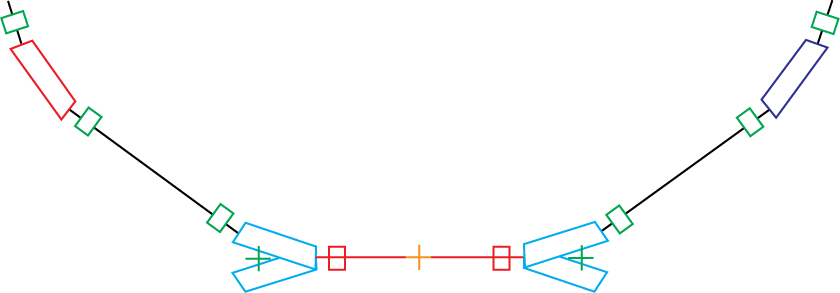
\includegraphics[width=.9\textwidth]{illustrations/misalign-fig1}
  \caption{Example 0: girder.}
  \label{fig:Example-0}
\end{figure}

On the image in \fref{Example-0}, the red and the cyan magnets
are part of a single girder. The origin of the girder frame of reference is
located in the middle of the red drift and displayed with an orange cross.

\index{rotation!order of}
%
The cyan magnets form two siamese: one on the left and one on the
right. The array \ptc{MIS(1:6)} contains the actual misalignments: the translations
in \ptc{MIS(1:3)} and the rotations in \ptc{MIS(4:6)}. They are applied in the
standard \PTC\ order: rotation around the $x$, then the $y$, and finally
the $z$-axis, followed by the translation.


\subsubsection*{Example 1}

Now we rotate the girder by 22.5 degrees, as shown in \fref{Example-1-1}.

\begin{figure}[ht]
  \centering
  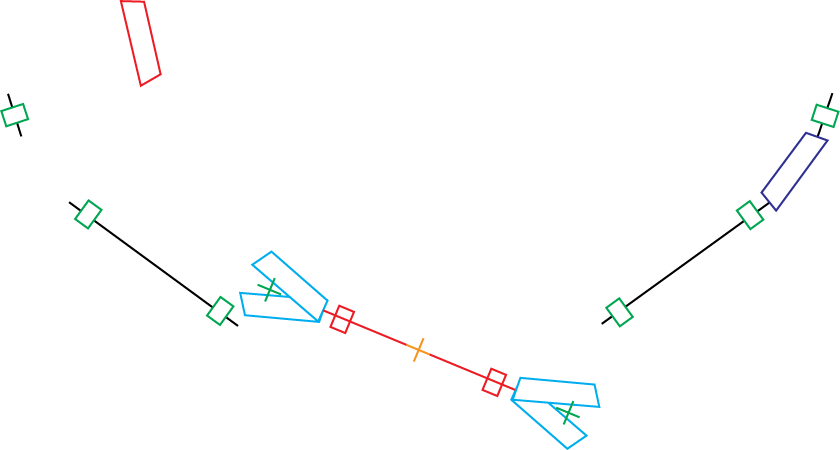
\includegraphics[width=.9\textwidth]{illustrations/misalign-fig2}
  \caption{Example 1: girder after 22.5 degree rotation.}
  \label{fig:Example-1-1}
\end{figure}

This was done with the command:

\begin{ptccode}
MIS=0.d0
MIS(5)=PI/8.d0
CALL MISALIGN_GIRDER(B,MIS,ADD=.FALSE.)
\end{ptccode}

If we follow this command by:

\begin{ptccode}
MIS=0.d0
MIS(1)=2.d0
CALL MISALIGN_GIRDER(B,MIS,ADD=.TRUE.)
\end{ptccode}

The \ptc{ADD=.TRUE.} indicates that the second misalignment of the girder
is additive. The misalignment is in the direction of the rotated girder,
as shown in \fref{Example-1-2}.

\begin{figure}[ht]
  \centering
  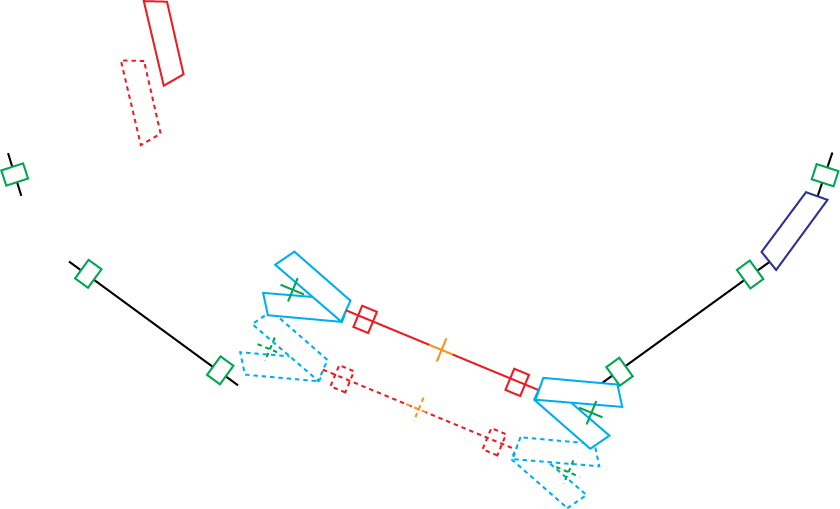
\includegraphics[width=.9\textwidth]{illustrations/misalign-fig3}
  \caption{Example 1: girder after an additive misalignment.}
  \label{fig:Example-1-2}
\end{figure}


\subsubsection{MISALIGN\_SIAMESE}

\index{routine!\ptc{MISALIGN\_SIAMESE}}
\index{MISALIGN\_SIAMESE@\ptc{MISALIGN\_SIAMESE}!routine}
%
\begin{ptccode}
MISALIGN_SIAMESE(S2,S1\textit{\textcolor{red}{,OMEGA,BASIS,ADD,PRESERVE_GIRDER}})
\end{ptccode}


\subsubsection*{Example 2}

Let us consider the following sequence of calls where the fibre pointer
\ptc{B} is pointing to a member of the left siamese:

\begin{ptccode}
MIS=0.d0
MIS(1)=2.d0
CALL MISALIGN_SIAMESE(B,MIS,ADD=.FALSE.)
MIS=0.d0
MIS(1)=2.d0
MIS(5)=PI/8.d0
CALL MISALIGN_GIRDER(B,MIS,ADD=.TRUE.)
\end{ptccode}

\fref[c]{Example-2} shows the result.

\begin{figure}[ht]\forceversofloat
  \centering
  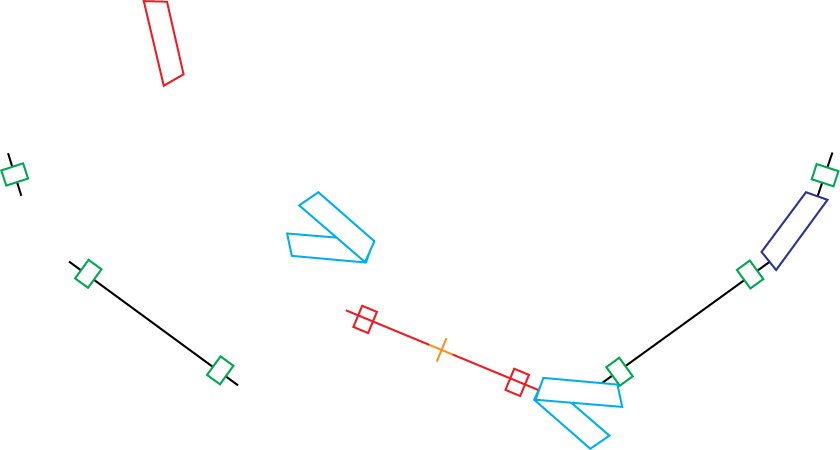
\includegraphics[width=.9\textwidth]{illustrations/misalign-fig4}
  \caption{Example 2: misalign siamese followed by misalign girder.}
  \label{fig:Example-2}
\end{figure}


\subsubsection*{Example 3}

Now let us switch the order.

\begin{ptccode}
MIS=0.d0
MIS(1)=2.d0
MIS(5)=PI/8.d0
CALL MISALIGN_GIRDER(B,MIS,ADD=.FALSE.)
MIS=0.d0
MIS(1)=2.d0
CALL MISALIGN_SIAMESE(B,MIS,ADD=.FALSE.)
\end{ptccode}

Here we purposely made \ptc{ADD=.FALSE.} on the siamese call since
naively one expects the position to be relative to the girder on which it
is attached. The results should be the same, but they are not---as we see
in \fref{Example-3}.

\begin{figure}[ht]
  \centering
  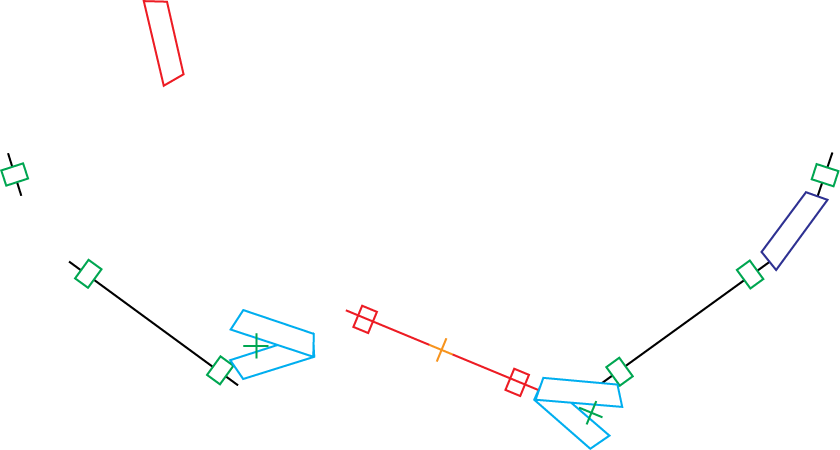
\includegraphics[width=.9\textwidth]{illustrations/misalign-fig5}
  \caption{Example 3: misalign girder followed by misalign siamese.}
  \label{fig:Example-3}
\end{figure}

All the magnets store their effective misalignments in one array.
Therefore the siamese has no knowledge of being on a girder.
 \ptc{ADD=.FALSE.} sends the siamese back to its original fibre.


\subsubsection*{Example 4}

This command avoids sending the siamese back to its original fibre 
prior to the misalignment:

\begin{ptccode}
MIS=0.d0
MIS(1)=2.d0
CALL MISALIGN_SIAMESE(B,MIS,ADD=.FALSE.,PRESERVE_GIRDER=.TRUE.)
\end{ptccode}

\fref[c]{Example-4} shows the result.

\begin{figure}[ht]
  \centering
  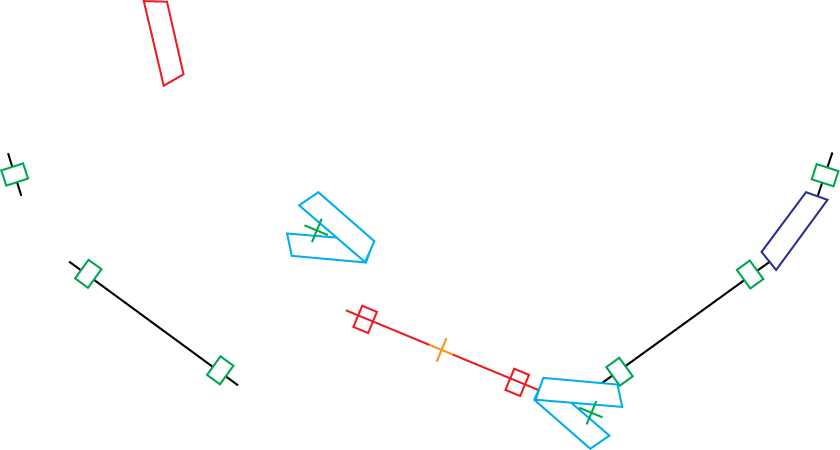
\includegraphics[width=.9\textwidth]{illustrations/misalign-fig6}
  \caption{Example 4: misalign siamese with \ptc{preserve\_girder=.true.}}
  \label{fig:Example-4}
\end{figure}

The same command with \ptc{MIS=0.d0} in the siamese always returns the siamese
to its girder position, not to fibre position.


\subsubsection{MISALIGN\_FIBRE}

\index{routine!\ptc{MISALIGN\_FIBRE}}
\index{MISALIGN\_FIBRE@\ptc{MISALIGN\_FIBRE}!routine}
%
This routine behaves like the siamese routine but acts on a single fibre.

\begin{ptccode}
MISALIGN_FIBRE(S2,S1\textit{\textcolor{red}{,OMEGA,BASIS,ADD,PRESERVE_GIRDER}})
\end{ptccode}

Note: If the \ptc{MISALIGN\_FIBRE} routine is used on a siamese, it mildly
breaks the siamese. One can imagine very tiny errors internal to a
siamese and bigger errors on the siamese and yet bigger errors on
a girder containing siamese and individual elements.

Therefore the following sequence of commands is acceptable if \ptc{B} is
an element part that is of a siamese and part of a girder:

\begin{ptccode}
CALL MISALIGN_FIBRE(B,MIS1)
CALL MISALIGN_SIAMESE(B,MIS2,ADD=.TRUE.)
CALL MISALIGN_GIRDER(B,MIS3,ADD=.TRUE.)
\end{ptccode}

Here we would imagine \ptc{MIS1} < \ptc{MIS2} < \ptc{MIS3}. Notice that 
\ptc{ADD=.TRUE.} on a siamese does not break a girder.

\begin{ptccode}
CALL MISALIGN_GIRDER(B,MIS3)
CALL MISALIGN_SIAMESE(B,MIS2,ADD=.FALSE. ,PRESERVE_GIRDER=.TRUE.)
CALL MISALIGN_FIBRE(B,MIS1,ADD=.TRUE.)
\end{ptccode}


\section{Dynamical Routines}
\fxnote{Review section title.}

\index{dynamical routines!described}
\index{routines!dynamical}
\index{Euclidean group!discussed}
\index{dynamical group!discussed}
%
Dynamical routines perform geometric rotations and translations, which act on the
tracked object itself. \PTC\ has an ``exact'' dynamical group and an ``approximate''
dynamical group. It is remarkable that the approximate dynamical rotations and
translations also form a group---but it is not isomorphic to the affine Euclidean group.

The ultimate goal of \PTC\ is to propagate particles and maps thanks to Taylor
polymorphism. Placing geometric objects in three dimensions is worthless unless
our rotations and translations can be translated into dynamical equivalents acting
on rays (and on spin).

\index{Lie algebra!discussed}
%
It is useful first to look at the Lie algebra acting on the $t$-based dynamics because it
contains within it as a subgroup the affine part discussed above.


\subsection{Exact Patching and Exact Misalignments: Dynamical Group}

\index{affine frame!dynamical group}
\index{patching!exact}
\index{misalignment!exact}
%
\PTC\ first computes patching and misalignments geometrically. The connection
between two affine frames is always expressed as follows through pure
geometric computations:
\begin{equation*}
  \text{Connection} = T(d_x,d_y,d_z) \circ R_z \circ R_y \circ R_x
\end{equation*}

This product of operators is in the usual matrix ordering. Therefore
the rotation in the $x$-axis acts first, followed by the $y$-axis, etc.
The rotations are computed using \ptc{COMPUTE\_ENTRANCE\_ANGLE}.

We factor the rotation in that manner because the operators R$_{x}$
and R$_{y}$ are drifts in polar coordinates and are therefore nonlinear.
For example, the rotation R$_{y}$ is a pole face rotation, dubbed
``prot'' by Dragt in the code MARYLIE. The formula is given by:

\begin{align*}
  \overline{x} &=
    \frac{x}{\cos\alpha\left(1-\frac{p_x}{p_z}\tan\alpha\right)},
    \text{ where }
    p_z = \sqrt{\left(1-\frac{2}{\beta_0}p_t + p_t^2\right)
                - p_x^2 - p_y^2} \\
  \overline{p}_x &= p_x\cos\alpha + p_z\sin\alpha \\
  \overline{y} &= y
    + \frac{x p_y\tan\alpha}%
           {p_z\left(1-\frac{p_x}{p_z}\tan\alpha\right)} \\
  \overline{p}_y &= p_y\\
  \overline{t} &=  t
    + \frac{x\left(\frac{1}{\beta_0}-p_t\right)\tan\alpha}%
           {p_z\left(1-\frac{p_x}{p_z}\tan\alpha\right)} \\
  \overline{p}_t &= p_t
\end{align*}

Here $(t,p_t)$ form a canonical pair.  In \PTC\ $(-p_t,t)$ form a canonical pair.

We get the rotation $R_x$ from $R_y$ by interchanging $x$ and $y$. Both
rotations rotate the magnet towards the direction of propagation, that is,
towards the $z$-direction.

The rotation $R_z$ is the usual affine rotation along the $z$-axis.
It is linear and transforms $(x,y)$ and $(p_x,p_y)$ identically,
leaving $(t,p_t)$ untouched.  It rotates the $x$-axis of the magnet
towards its $y$-axis.

\index{Lie operators!discussed}
%
The Lie operators for the three translations and rotations are given by:
\begin{align*}
  \lieop{T_x} &= \lieop{p_x}, \\
  \lieop{T_x} &= \lieop{p_x}, \\
  \lieop{T_y} &= \lieop{p_y}, \\
  \lieop{T_z} &= \Lieop{\sqrt{(1+\delta)^2 - p_x^2 - p_y^2}}, \\
  \lieop{L_x} &= \Lieop{y\sqrt{(1+\delta)^2 - p_x^2 - p_y^2}}, \\
  \lieop{L_y} &= -\Lieop{x\sqrt{(1+\delta)^2 - p_x^2 - p_y^2}}, \\
  \lieop{L_z} &= \lieop{xp_y - yp_x}.
\end{align*}
It is remarkable that these Lie operators have the same Lie algebra
as the ordinary affine (or time) Lie operators:
\begin{alignat*}{3}
  [L_x, L_y] &= L_z, &\qquad [L_x, p_y] &= p_z, &\qquad [L_x, p_z] &= -p_y,\\
  [L_y, L_z] &= L_x, &\qquad [L_y, p_z] &= p_x, &\qquad [L_y, p_x] &= -p_z,\\
  [L_z, L_x] &= L_y, &\qquad [L_z, p_x] &= p_y, &\qquad [L_z, p_y] &= -p_x.
\end{alignat*}
The Lie groups are therefore locally isomorphic.  Of course one notices
that ``prot'' ($R_x$ and $R_y$) has a divergence at $\alpha=90^\circ$.
It is not possible in the ``lens'' or ``s'' paradigm to rotate a magnet map 
by $90^\circ$ and get meaningful propagators. Therefore the dynamical
group is locally isomorphic.


\subsection{Inexact Patching and Exact Misalignments}

\index{patching!inexact}
\index{misalignment!inexact}
\index{Euclidean group!pseudo}
\index{pseudo-Euclidean group!discussed}
%
\PTC\ provides for an emasculated pseudo-Euclidean group. The Lie operators
are obtained by expanding the dynamical maps keeping the energy dependence
exact. This is in tune with the \ptc{exact\_model=false} option.
\begin{align*}
  \lieop{T_x} &= \lieop{p_x}, \\
  \lieop{T_y} &= \lieop{p_y}, \\
  \lieop{T_z(r_1,r_2)}
    &= \lieop{\mhsp r_1
              \underbrace{\Bigl(-\frac{p_x^2+p_y^2}{1(1+\delta)}\biggr)}_{D_z}
              + r_2\delta\mhsp}, \\
  \lieop{L_x} &= \lieop{y(1+\delta)}, \\
  \lieop{L_y} &= -\lieop{x(1+\delta)}, \\
  \lieop{L_z} &= \lieop{xp_y - yp_x}.
\end{align*}
This group has seven generators for convenience. The Lie algebra differs
from the original algebra of the Euclidean group as follows:
\begin{align*}
[L_x, L_y] &= 0,\\
[L_x, p_y] &= T_z(0,1) = \text{emasculated} p_z,\\
[L_y, p_x] &= -T_z(0,1).
\end{align*}

Why do we care about the approximate Euclidean group?

The reason is speed: if a fast post-processor to \PTC\ is written. Let
us assume that we have represented a (large) machine with \ptc{exact\_model=false}
and the drift-kick-drift option. \fref[c]{Pseudo-Euclidean-maps}
schematically shows two magnets separated by a drift.

\begin{figure}[ht]
  \centering
  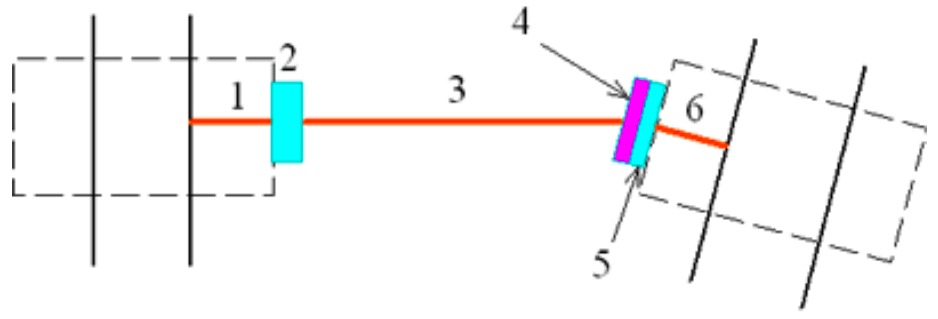
\includegraphics[width=.9\textwidth]{illustrations/pseudo-Euclidean-maps}
  \caption{Pseudo-Euclidean maps.}
  \label{fig:Pseudo-Euclidean-maps}
\end{figure}

The drifts (1,3,6) are in red. Some of the drifts (1,6) are part
of the integration scheme. The misalignments are made of our six
pseudo-Euclidean operators; they are in cyan (2,4). Finally a patch (4)
is needed; it is in magenta.

The blue and cyan operators contain our six pseudo-Euclidean maps.
Therefore to go from 1 to 6 in the figure may involve over 20 maps.
By using the group properties, this can be reduced to six maps!

\fxnote{What does the ``blue'' in ``blue and cyan operators'' refer to? I see red, cyan, and magenta but no blue.}

